\documentclass[10pt,a4paper]{book}
\usepackage[utf8]{inputenc}
\usepackage[spanish]{babel}
\usepackage{amsmath}
\usepackage{amsfonts}
\usepackage{amssymb}
\usepackage{graphicx}
\usepackage[left=2cm,right=2cm,top=2cm,bottom=2cm]{geometry}
\usepackage{hyperref}
\hypersetup{
    colorlinks=true,
    linkcolor=cyan,
    anchorcolor=cyan,
    filecolor=cyan,
    urlcolor=blue,
}

%Header and footer customized
\usepackage{fancyhdr}
\pagestyle{fancy}

\usepackage{xcolor}
\usepackage{titling}

\usepackage{listingsutf8}
\usepackage{listings}
\usepackage{color}


%New colors defined below
\definecolor{codegreen}{rgb}{0,0.6,0}
\definecolor{codegray}{rgb}{0.5,0.5,0.5}
\definecolor{codepurple}{rgb}{0.58,0,0.82}
\definecolor{backcolour}{rgb}{0.95,0.95,0.92}

%Code listing style named "mystyle"
\lstdefinestyle{mystyle}{
  backgroundcolor=\color{backcolour},   commentstyle=\color{codegreen},
  keywordstyle=\color{magenta},
  numberstyle=\color{codegray},
  stringstyle=\color{codepurple},
  basicstyle=\scriptsize\ttfamily\tiny,
  breakatwhitespace=false,         
  breaklines=true,                 
  captionpos=b,                    
  keepspaces=true,                                     
  numbersep=5pt,                  
  showspaces=false,                
  showstringspaces=false,
  showtabs=false,                  
  tabsize=2,
  framextopmargin=1pt,
  framexbottommargin=10pt,
}

\usepackage{sectsty}
\partfont{\large}

%"mystyle" code listing set
\lstset{style=mystyle}

%For generate graphs
\usepackage{pgf}
\usepackage{tikz}
\usetikzlibrary{arrows,automata}

% To generate a box with text and background
\definecolor{shadecolor}{RGB}{200,201,190}
\newcommand{\mybox}[1]{\par\noindent\colorbox{shadecolor}
{\parbox{\dimexpr\textwidth-2\fboxsep\relax}{#1}}}

\author{Ruben Vasallo Gonzalez}
\title{PROYECTO FINAL MÁSTER \\ CLASIFICADOR DOCUMENTOS MÉDICOS HOPE \\ 2020 - 2021}

%header
\headsep = 1,5cm
\lhead{\begin{picture}(0,0) \put(0,0){
\includegraphics[width=2cm]{logo-uoc-default.png}} \end{picture}}
\chead{}
\rhead{\thetitle \\ \theauthor}

%footer
\lfoot{}
\cfoot{\thepage}
\rfoot{}

%set head of page
\setlength{\textheight}{230mm}

\begin{document}
\maketitle

\tableofcontents

\part{Objetivo del Proyecto}

\chapter{Introducción}

\section{Definición del proyecto y objetivo}

\paragraph{}
El proyecto de fin de máster nace de la necesidad de clasificar y recomendar resultados sobre estudios clínicos de confianza y actualizados. En Internet existe muchísima información sobre medicina y salud y no siempre toda es de fiar.

\paragraph{}
Actualmente existen bases de datos de confianza en donde los científicos y el publico en general puede buscar informes sobre estudios clínicos desarrollados anteriormente, pero no siempre es fácil o rápido encontrar estos resultados.

\paragraph{}
Actualmente existe el proyecto HOPE, donde médicos de todo el mundo puede consultar en una base de datos informes médicos relacionados con los síntomas que puedan tener sus pacientes y ver que otros tratamientos han dado resultado. Todo y con eso, el sistema no siempre devuelve los artículos más relevantes o actualizados por lo que, no siempre la información consultada es útil.

\paragraph{}
En este ámbito, los profesionales médicos pueden valorar si la información recibida ha sido útil o no respecto a la búsqueda que han realizado, por lo que con ese \textit{feedback}, se pretende crear un recomendador que aproxime mejor los resultados a las búsquedas realizadas.

\paragraph{}
Con todo esto, el objetivo que se pretende alcanzar en este proyecto es el de entrenar un modelo predictivo que sea capaz de discriminar en base a los términos buscados por el medico, cuales son los mejores artículos útiles que pueden ayudar a resolver el problema.

\section{Que es el proyecto HOPE}

\paragraph{}
El proyecto HOPE (que significa \textit{Health Operations for Personalized Evidence} en ingles) nace de la necesidad de ayudar a los científicos médicos a encontrar la información que necesitan de la manera más rápida y fácil posible. Existe infinidad de información medica en Internet de miles de proyectos investigados y esto hace que, muchas veces sea complicado encontrar la información sobre ensayos médicos para tratar información. En el ámbito de la medicina el tiempo perdido puede costar vidas y es un precio demasiado elevado a pagar, tanto a nivel económico como emocional.

\paragraph{}
El proyecto HOPE es un sistema basado en inteligencia artificial para identificar los datos claves de casos clínicos registrados en la Historia Clínica Electrónica, en base a los cuales realiza una búsqueda única por paciente para proporcionar al profesional de la salud recomendaciones de tratamientos, estudios de investigación, información para el paciente, todo en base a registros de fuentes científicas de información.


\chapter{Extracción y procesado de datos}

\section{Extracción}

\paragraph{}
El Origen de los datos se encuentra en una Base de datos SQL distribuida en dos tablas, que pasamos a detallar a continuación:

\paragraph{• Tabla \textit{fed\_hope\_sugerencia}}

\paragraph{}
\begin{figure}[h]
  \centering
  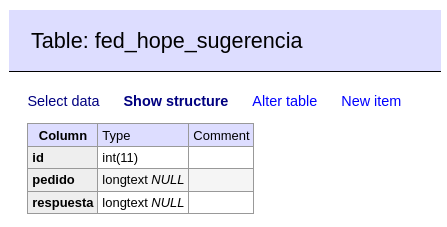
\includegraphics[width=8cm]{images/extraccion_1_1.png}
  \caption{Visualización de los atributos de la tabla \textit{fed\_hope\_sugerencia}}
\end{figure}

\paragraph{}
En esta tabla encontraremos la sugerencia que dio el programa HOPE en base a los parámetros que introdujo el usuario, almacenado en el atributo pedido y la respuesta que dio el programa, almacenado en el atributo respuesta. Todos los datos son almacenados en formato json.

\newpage
\paragraph{\textbf{Atributo pedido}: } Si analizamos el formato de datos que tenemos del atributo pedido observamos los siguientes atributos:

\lstset{inputencoding=utf8/latin1}
\lstinputlisting[frame=single]{codes/extraccion_1_1.json}

\paragraph{}
Podemos ver varios atributos haciendo referencia a los síntomas que consulta el profesional medico.

\paragraph{\textbf{Atributo respuesta}: } En el atributo respuesta obtenemos entre otros datos, el listado de artículos científicos sugeridos relacionados con los síntomas descritos por el profesional medico. Esta respuesta es muy amplia pero entre todos los atributos, podemos observar un listado de ids de artículos, con sus fechas de revisión de estos artículos y unas claves descriptivas para esos artículos.

\paragraph{}
\textbf{Nota:} Mostramos una pequeña parte del contenido de una observación del atributo respuesta.
\begin{figure}[h]
  \centering
  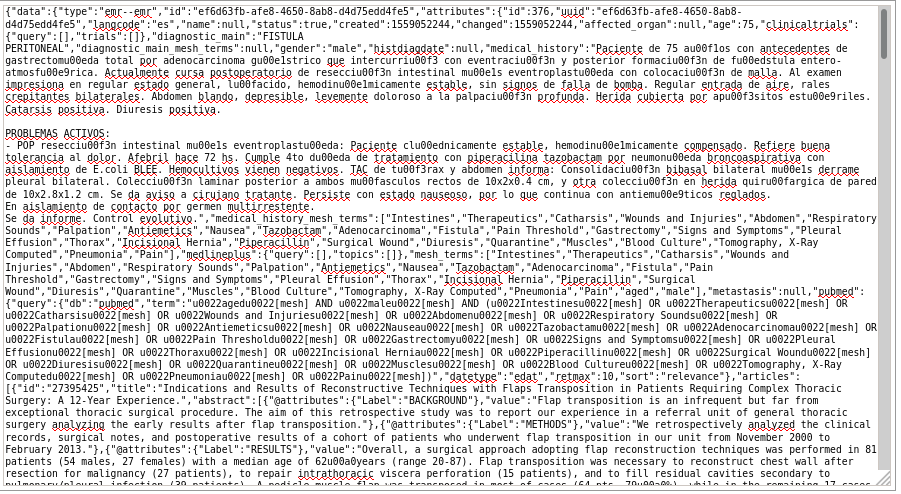
\includegraphics[width=8cm]{images/extraccion_1_2.png}
  \caption{Ejemplo de contenido del atributo respuesta de una observación}
\end{figure}


\section{Procesado de datos}
TODO

\chapter{Análisis de los datos}

\section{Análisis de componentes principales}
TODO

\chapter{Aproximación de resultados}

\section{Aproximación por Vecinos más próximos (K-NN)}
TODO

\part{Objetivo del Proyecto}

\chapter{Modelos Predictivos}

\section{Regresión logística}
TODO

\part{Conclusiones}

\chapter{Resultados obtenidos}
TODO

\end{document}